\documentclass[paper=letter, fontsize=11pt]{scrartcl} 
 \usepackage[top=2.5cm, bottom=2.5cm, left=2.5cm, right=2.5cm]{geometry}
\usepackage{framed}

\usepackage{graphicx}
\usepackage{verbatim}
\usepackage{pictex}  
\usepackage{multimedia}
\usepackage{listings}
\usepackage{xcolor,colortbl}
\usepackage[spanish]{babel} % language/hyphenation
\usepackage{amsmath,amsfonts,amsthm} % Math packages
\usepackage{amsbsy}
\usepackage{amssymb}
\usepackage{fancyvrb}
\usepackage{sectsty} % Allows customizing section commands
\usepackage[dvipsnames]{xcolor}

\newcommand{\defi}[3]{\textbf{Definición:#3}}
\newcommand{\fin}{$\blacksquare.$}
\newcommand{\finf}{\blacksquare.}

\newcommand{\grstep}[2][\relax]{%
   \ensuremath{\mathrel{
       {\mathop{\longrightarrow}\limits^{#2\mathstrut}_{
                                     \begin{subarray}{l} #1 \end{subarray}}}}}}
\newcommand{\swap}{\leftrightarrow}

\newcommand{\gen}{\text{gen}}

\newtheorem{thmt}{Teorema:}
\newtheorem{thmd}{Definición:}
\newtheorem{thml}{Lema:}
\newtheorem{thmj}{Ejemplo:}
\newtheorem{thma}{Algoritmo:}
\newtheorem{thmp}{Propiedad:}


\newcommand{\mub}{\mathbf{\mu}}
\newcommand{\Sb}{\mathbf{S}}
\newcommand{\mb}{\mathbf{m}}
\newcommand{\cb}{\mathbf{c}}
\newcommand{\xb}{\mathbf{x}}
\newcommand{\Xb}{\mathbf{X}}
\newcommand{\yb}{\mathbf{y}}
\newcommand{\Yb}{\mathbf{Y}}
\newcommand{\Simgab}{\mathbf{\Sigma}}
\newcommand{\sumk}{\sum_{k=1}^K}
\newcommand{\sumi}{\sum_{i=1}^n}
\newcommand{\sumj}{\sum_{j=1}^n}
\usepackage{biblatex}
\addbibresource{biblio.bib}

\allsectionsfont{\centering \normalfont\scshape} % Make all sections centered, the default font and small caps
\usepackage{float}
\usepackage{fancyhdr} % Custom headers and footers
\pagestyle{fancyplain} % Makes all pages in the document conform to the custom headers and footers
\fancyhead{} % No page header - if you want one, create it in the same way as the footers below
\fancyfoot[L]{} % Empty left footer
\fancyfoot[C]{} % Empty center footer
\fancyfoot[R]{\thepage} % Page numbering for right footer
\renewcommand{\headrulewidth}{0pt} % Remove header underlines
\renewcommand{\footrulewidth}{0pt} % Remove footer underlines
\setlength{\headheight}{13.6pt} % Customize the height of the header
\usepackage{biblatex}
\addbibresource{references.bib}
\numberwithin{equation}{section} % Number equations within sections (i.e. 1.1, 1.2, 2.1, 2.2 instead of 1, 2, 3, 4)
\numberwithin{figure}{section} % Number figures within sections (i.e. 1.1, 1.2, 2.1, 2.2 instead of 1, 2, 3, 4)
\numberwithin{table}{section} % Number tables within sections (i.e. 1.1, 1.2, 2.1, 2.2 instead of 1, 2, 3, 4)

\setlength\parindent{0pt} % Removes all indentation from paragraphs - comment this line for an assignment with lots of text

\newcommand{\horrule}[1]{\rule{\linewidth}{#1}} % Create horizontal rule command with 1 argument of height

\title{	
\normalfont \normalsize 
\textsc{Centro de Investigaci\'on en Matem\'aticas (CIMAT). Unidad Monterrey} 
\\ [25pt] 
\horrule{0.5pt} \\[0.4cm] % Thin top horizontal rule
\huge Tarea 5 \\ 
\horrule{2pt} \\[0.5cm] % Thick bottom horizontal rule
}


\author{Enrique Santibáñez Cortés} % Your name

\date{\normalsize\today} % Today's date or a custom date

\begin{document}
\lstdefinestyle{customc}{
  belowcaptionskip=1\baselineskip,
  basicstyle=\footnotesize, 
  frame=lrtb,
  breaklines=true,
  %frame=L,
  %xleftmargin=\parindent,
  language=C,
  showstringspaces=false,
  basicstyle=\footnotesize\ttfamily,
  keywordstyle=\bfseries\color{green!40!black},
  commentstyle=\itshape\color{red!40!black},
  identifierstyle=\color{blue},
  stringstyle=\color{purple},
}

\lstset{breakatwhitespace=true,
  basicstyle=\footnotesize, 
  commentstyle=\color{green},
  keywordstyle=\color{blue},
  stringstyle=\color{purple},
  language=C++,
  columns=fullflexible,
  keepspaces=true,
  breaklines=true,
  tabsize=3, 
  showstringspaces=false,
  extendedchars=true}

\lstset{ %
  language=R,    
  basicstyle=\footnotesize, 
  numbers=left,             
  numberstyle=\tiny\color{gray}, 
  stepnumber=1,              
  numbersep=5pt,             
  backgroundcolor=\color{white},
  showspaces=false,             
  showstringspaces=false,       
  showtabs=false,               
  frame=single,                 
  rulecolor=\color{black},      
  tabsize=2,                  
  captionpos=b,               
  breaklines=true,            
  breakatwhitespace=false,    
  title=\lstname,             
  keywordstyle=\color{blue},  
  commentstyle=\color{dkgreen},
  stringstyle=\color{mauve},   
  escapeinside={\%*}{*)},      
  morekeywords={*,...}         
} 

\maketitle

\section{Clasificación de los datos MNIST (remasterizado)}
\subsection{Introducción}
En el contexto del ejercicio 2 de la tarea 5 de este curso, en este ejercicio intentaremos aplicar diferentes  (a los de la tarea pasada) métodos de clasificación con el objetivo de poder clasificar las imágenes en los dígitos que aparecen en ellas. Para ello utilizaremos $K-Fold$ CV como criterio para elegir el mejor modela, así como para compararlos. En todos los modelos se consideraron 4-fold.


\subsection{Actualización del Bets model}
Anteriormente habíamos concluído que el mejor modelo aplicada fue \textbf{utilizando el modelo QDA a una representación de los datos basada en PCA considerando los primeros 200 componentes principales.} Pero este resultado fue sin utilizar validación cruzada, por lo que es necesario actualizarlo.\\

\textbf{Utilizando solamente los datos de entrenamiento}, consideramos \textbf{4-fold} y probamos el rendimiento de diferentes número de componentes principales: \textbf{50, 80, 100, 200}. La métrica que consideramos correcta fue el acuaracy debido a que es una métrica general del rendimiento del ajuste, pero con la precaución de que puede ser engañosa en algunos problemas.\\

Se ocuparon las funciones \textit{Pipeline y GridSearchCV} para los ajustes considerando validación cruzada. El score promedio de los 4-fold para los 4 modelos ajustados se muestran en la \textbf{Figura \ref{qda_best_model}}, y de la cual podemos concluir que el mejor modelo es considerando la \textbf{representación de los 50 componentes principales con un score de 0.96}. Algo interesante a resaltar, es que cuando más componentes principales utilizamos el rendimiento en este modelo va decreciendo.

\begin{figure}[H] 
\centering
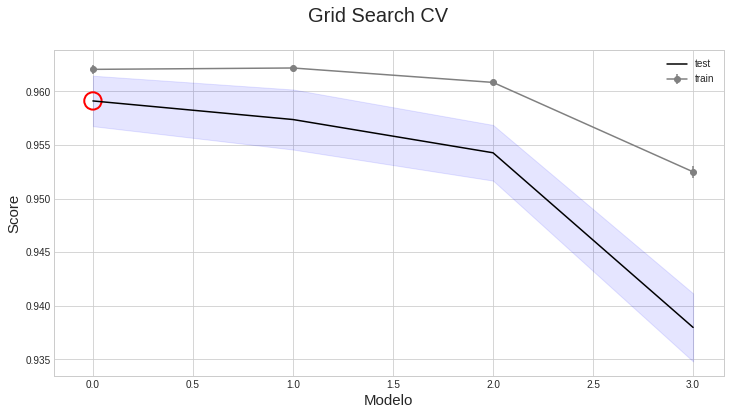
\includegraphics[scale=0.5]{figure/best_model_update.png}\caption{Score usando K-fold CV y el modelo QDA.}\label{qda_best_model}
\end{figure}

\subsection{Nuevos modelos de clasificación}
Los nuevos métodos de clasificación considerados son basados en: Redes neuronales, Máquinas de Soporte Vectorial(SVM), Arboles de clasificación(tree) y AdaBoost. \textbf{Cabe mencionar que se utilizo una representación de los datos usando PCA, debido a que el costo computacional de usar todos los datos era muy grande,} consideramos diferentes número de componentes principales: \textbf{50, 80, 200}.\\

Cada método de clasificación tiene diferentes hiperparametros a controlar, para cada uno de ellos consideramos algunos de los más importates y el resto tomaron el valor \textit{default} que tiene las funciones de sklearn \cite{scikit-learn} ocupadas.

\subsubsection*{Redes Neuronales}
Consideramos diferentes arquitecturas para las redes neuronales: \textbf{una capa oculta y una neuronal, diez capaz ocultas cada una con una neurona, diez capaz ocultas con diez neuronas y diez capas ocultas con tres neuronas}. También se consideraron diferentes valores para el parámetro de regularización: \textbf{0.1, 0.5 y 0.01}; y también consideramos diferentes funciones de activación: \textbf{identity, logistic, tanh y relu}. En total se probaron 58 modelos distintos, se probaron primero 35 modelos y posteriormente 23 debido al costo computacional.\\

Los resultados se pueden observar en las Figuras \ref{redes}. Podemos observar que la función de activación usando \textit{logistic, tanh y relu} no tienen mucha diferencias entre sí, pero la función de activación \textit{relu} si y fue la mejor de ellas. Después de esta conclusión, procedimos a buscar la mejor arquitectura de la red (ver Figura \ref{arqui}). La mejor combinación de parametros fue considerando \textbf{diez capas ocultas con diez neuronas cada una usando la función de activación relu con un valor de 1 en el parámetro de regularización y utilizando los primeros 200 componentes principales, la cual arrojo un score de 0.89.}

\begin{figure}[!htb]
\minipage{0.5\textwidth}
  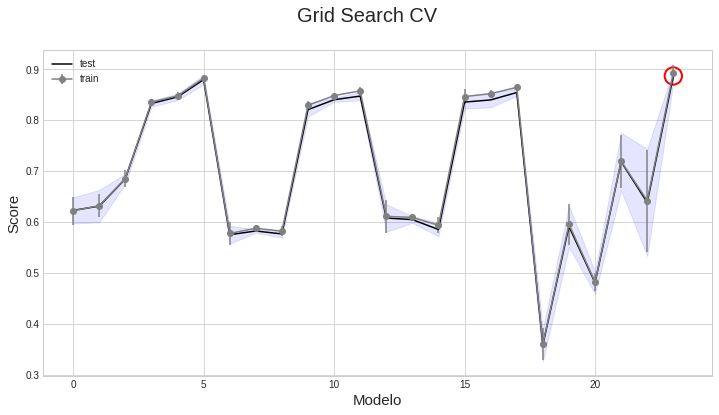
\includegraphics[width=\linewidth]{figure/redes_neuronales_2.png}
  \caption{Efecto de la función de activación.}\label{act}
\endminipage\hfill
\minipage{0.5\textwidth}
  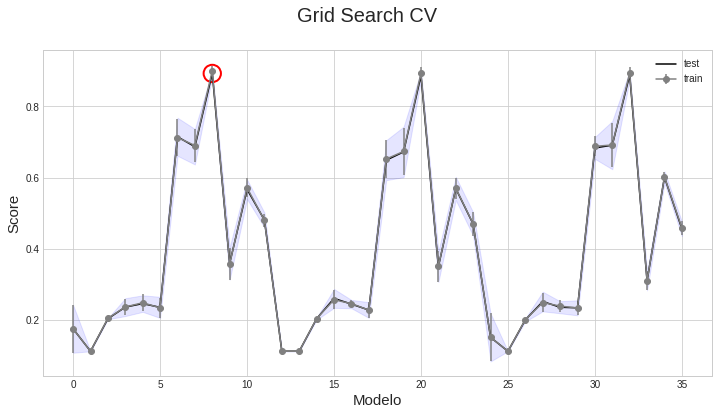
\includegraphics[width=\linewidth]{figure/redes_neuronales.png}\caption{Efecto de la arquitectura de la read.}\label{arqui}
\endminipage
\caption{Score usando K-fold CV y usando redes neuronales.}\label{redes}
\end{figure}


\subsubsection*{SVM}
Para este modelo los hyperparametros a controlar fueron el parametro de regularización: \textbf{0.001, 0.01 y 1};   el tipo kernel usando en el algoritmo: \textbf{linear y rbf}; y el coeficiente del kernel (cuando use un kernel rbf): 0.001, 0.01, 0.1, 1, 10 y 100. En total se probaron 63 modelos.\\

Los resultados de la validación cruzada se observa en la Figura \ref{svm}. Podemos observar que cuando utilizamos un kernel \textit{rbf} el modelo es malo en comparación con un kernel \textit{linear}. Ahora considerando solo los modelos con un kernel \textit{linear}, podemos observar que entra mayor sea el número de componentes principales a usar el rendimiento es mayor. El efecto del  parámetro de regularización no es tan grande como los otros parámetros considerados. 

\begin{figure}[H] 
\centering
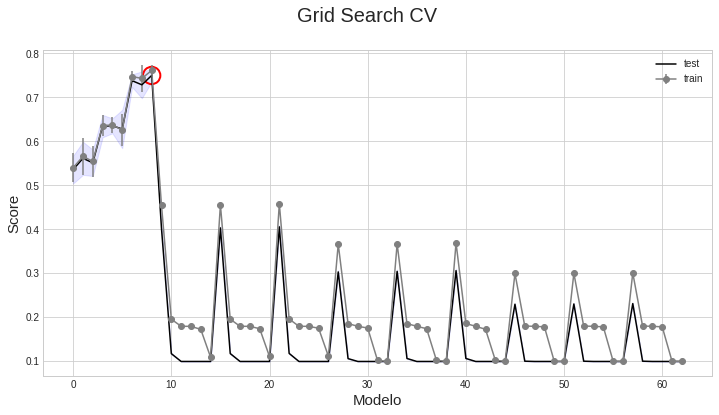
\includegraphics[scale=0.4]{figure/SVM.png}\caption{Score usando K-fold CV y el modelo SVM.}\label{svm}
\end{figure}

\textbf{La mejor combinación de hiperparametros es considerar un kernel linear con un valor de 1 en el parametro de regularización y utilizando una representación de 200 componentes principales de los datos, el cual arroja un score de 0.75.} 


\subsubsection*{Arboles de clasificación}
Para este modelo los hyperparametros a controlar fueron el número de hojas de los arboles: \textbf{2, 3 y 5},  y el número de variables a considerar para realizar la mejor separación: \textbf{auto, sqrt y log2}. En total se probaron 27 modelos.\\

Los resultados de la validación cruzada se observa en la Figura \ref{tree}. Para este modelo se observar un efecto muy notoria para los tres parámetros considerados, pero lamentablemente el \textbf{escore máximo de todas las combinaciones posibles es de $0.438116$ lo cual es muy malo, el cuál se obtiene utilizando 3 hojas en los arboles y usando el valor auto.}

\begin{figure}[H] 
\centering
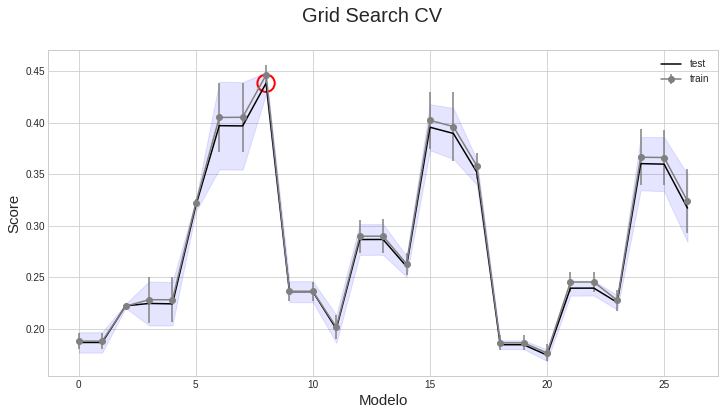
\includegraphics[scale=0.5]{figure/tree.png}\caption{Score usando K-fold CV y utilizando Decision tree.}\label{tree}
\end{figure}


\subsubsection*{AdaBoots}
Para este último modelo, los párametros más importantes son el clasificador débil y el número de iteraciones bosting y el algoritmo. Nosotros primero solo controlamos el número de iteraciones: 50, 100 y 200; y el algorimos a usar: SAMME y SAMME.R, estas combinaciones fijamos el clasificador base ocupado un arbol de desición una 1 hoja. Y posteriormente contralamos el clasificador base, el cual consideramos todas las combinaciones del clasificación de los Arboles de clasifiación de la sección anterior.\\

Primero obtuvimos que la mejor combinación de párametros fue ocupar \textbf{200 iteraciones con el algoritmo SAMME}. Posteriormente, fijando la combinación anterior y cambiando el clasificador base obtuvimos que la mejor combinación es considerando\textbf{ 3 hojas en los arboles de desición y considerar un número máximo de variables a considerar log2, esta combinación nos arrojo un score de 0.7795.}
\begin{figure}[H]
\minipage{0.5\textwidth}
 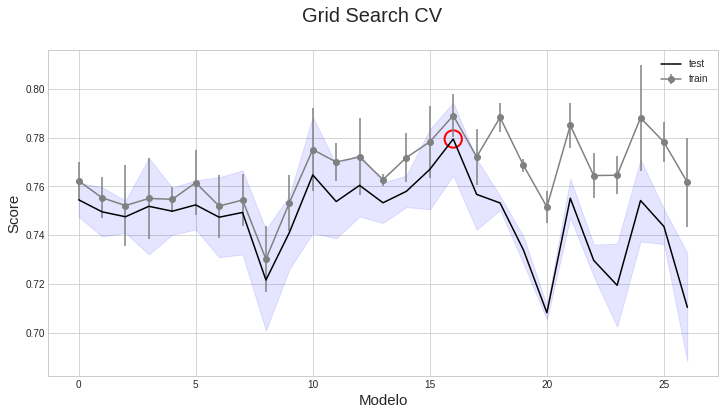
\includegraphics[scale=0.4]{figure/ada.png}\caption{Score usando K-fold CV y el modelo AdaBoots.}\label{ada}
\endminipage\hfill
\minipage{0.5\textwidth}
  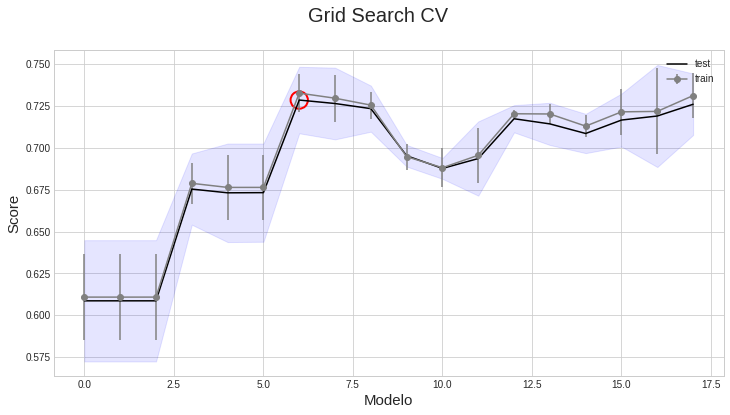
\includegraphics[scale=0.4]{figure/ada_2.png}\caption{Score usando K-fold CV y el modelo AdaBoots.}\label{ada2}
\endminipage
\caption{Score usando K-fold CV y usando AdaBoots.}\label{adas}
\end{figure}

Estaría interesante utilizar otro clasificador base, pero los arboles de desición son los \textit{menos costosos computacionalmente (de los que estamos probando).}

\subsection{Comparación de los mejores modelos}
Si comparamos todos los mejores scores de los diferentes modelos probados anteriormente (ver Cuadro \ref{compa}), podemos observar que \textbf{el mejor modelo se obtiene usando QDA y 50 componentes principales.} Es decir, nuestro modelo considerado en la tarea anterior tiene mejor rendimiento que los nuevos métodos aplicados. Además de que es el modelo más simple, en términos de parámetros y costo computacional. Esta última si tiene una gran diferencia con los nuevos métodos. 

\begin{table}[H]
\centering
\begin{tabular}{cccc}
\hline \hline
Model & score &Hiperparámetros &Datos \\
QDA & 0.96 & -&50 componentes principales\\
Redes neuronales & 0.89 &$[10,10],\ relu,\ C=1$&200 componentes principales\\
SVM & 0.75  &$linear, \ C=1$ &200 componentes principales\\
Arboles de clasificación & 0.4381 & $3, auto$& 50 componentes principales\\
ADABoots & 0.7795&$SAMME,\ 200,\ 3 \ hojas,\ log2$ &200 componentes principales  \\ \hline \hline 
\end{tabular}
\caption{Comparación de los score usando 4-fold.}\label{compa}
\end{table}
\subsection{Evaluación del mejor modelo en los datos de prueba.}
Dependiendo del problema, tener un score del 0.96 en el conjunto de prueba se puede considerar muy bueno. Pero igual depende de muchos factores: costo por cometer un error, frecuencia de los errores en una clasificación, etc. Pero en este caso yo podría concluir que el score obtenido es muy bueno. Entonces una vez seleccionado el mejor modelo, calculamos las métricas de error para el conjunto de prueba (ver Cuadro \ref{error}). Observando las metricas de error podemos notar que en general las métricas son muy buenas, la mayoría estan por arriba del 0.96. 
\begin{table}[H]
    \centering 
        \begin{tabular}{|c|c|c|c|c}
        \hline
dígito  & precision &  recall & f1$-$score\\
0       &  0.97  &  0.99   & 0.98\\  
1       &  1.00  &  0.97   & 0.98\\  
2       &  0.93  &  0.97   & 0.95\\  
3       &  0.96  &  0.96   & 0.96\\  
4       &  0.98  &  0.98   & 0.98\\  
5       &  0.97  &  0.97   & 0.97\\  
6       &  0.99  &  0.96   & 0.98\\  
7       &  0.98  &  0.93   & 0.96\\  
8       &  0.89  &  0.96   & 0.93\\  
9       &  0.97  &  0.94   & 0.95\\  \hline \hline
accuracy  & & & 0.96\\ \hline \hline
        \end{tabular}
        \caption{Métricas de error para el conjunto de prueba.} \label{error}  
\end{table}
Los números en donde hay más errores es considerando la clasificación del 8 (Ver Figura \ref{ocho}). En conclusión, podríamos decir que este ajuste es muy bueno para clasificar las imágenes de los dígitos.
\begin{figure}[H]
\centering
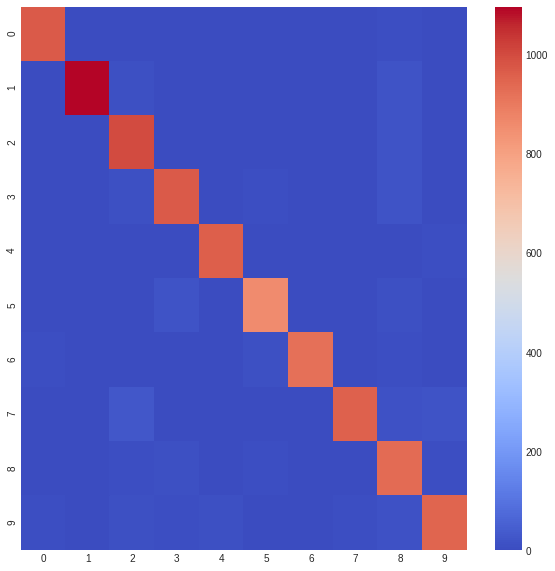
\includegraphics[scale=0.4]{figure/metric.png}
\caption{Matriz de confusión del conjunto de prueba, usando el mejor modelo QDA.}\label{ocho}
\end{figure}

Debido a que no pude contar con internet estos días, no pude acceder a Google Colab para probar más modelos y mi computadora no es muy eficiente. Me hubiera gustado jugar más con diferentes arquitecturas de redes neuronales, y me podría asegurar que es posible conseguir una mejor métrica de la obtenida en este trabajo usando QDA.

\section{Análisis de texto y de sentimientos (remasterizado)}
Recordando el ejercicio 3 d) de la tarea 5, el cuál tenía como objetivo poder ajustar un modelo para clasificar los textos según el tópico y el sentimiento. Recordemos para poder clasificar el tópico de un texto obtuvimos muy buenas métricas de error y para clasificar el sentimiento tuvimos métricas no tan buenas, \textbf{nos enfocaremos en implementar nuevos métodos de clasificación para el sentimiento}. Ya que (desde mi perspectiva) no tiene sentido aplicar métodos más complejos a problemas que tienen buenas métricas de error usando métodos más simples, \textit{lo simple es mejor}. \\

La representación BOW es la misma que se considero en la tarea 5, es decir, se considero tamaño de vocabulario igual a  \textit{V=3000} y consideramos un rango de (1,1) para los n-gramas. En la mayoría de los ajustes, consideramos la representación BOW completa y además consideramos una representación utilizando PCA, considerando distintos números de componenetes principales.\\

En las repuestas de la tarea 5 no utilizamos validación cruzada, por lo que primero actualizamos los modelos anteriores usando K-Fold CV. Y posteriormente apliquemos los nuevos métodos del ejercicio 1. En todos los modelos se consideraron 5-fold. 

\subsection*{Actualización de los modelos anterioes: LDA, QDA y Regresión Logística}

Para LDA y QDA, lo único que controlamos fue el número de componentes principales a utilizar: 30, 50, 60, 70, 200. Los resultados de la validación cruzada se pueden opservar en las Figuras \ref{s_lda} y \ref{s_qda}. \textbf{El mejor score de los 10 modelos probados fue 0.75, el cual se obtiene usando LDA en los primeros 60 componentes principales.}

\begin{figure}[!htb]
\minipage{0.5\textwidth}
  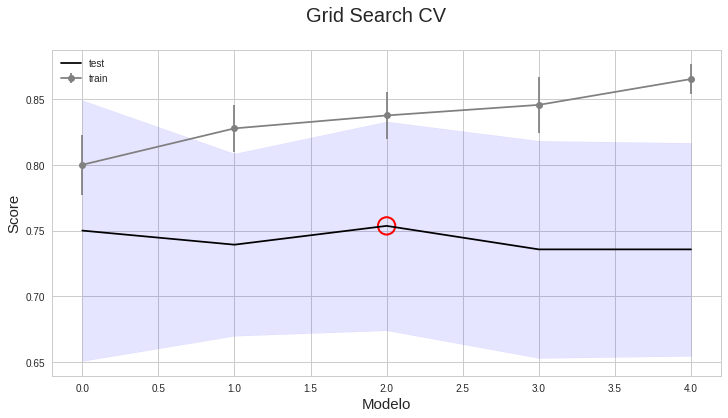
\includegraphics[width=\linewidth]{figure/s_lda_pca.png}\caption{Score K-Fold, LDA}\label{s_lda}
\endminipage\hfill
\minipage{0.5\textwidth}
  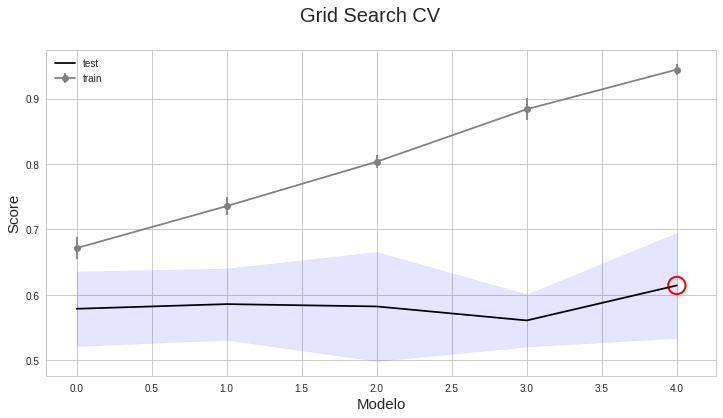
\includegraphics[width=\linewidth]{figure/s_qda_pca.png}
  \caption{Score K-Fold, QDA}\label{s_qda}
\endminipage
\end{figure}

Ahora, para el modelo de regresión logística (ver las Figuras \ref{s_reg}), consideramos el párametro $multi\_class$: ovr y multinomial; y distintos valores de regularización: 0.1, 0.05, 0.0094 y 0.005. \textbf{Y el mejor score de los 48 modelos probados fue de 0.7678, el cual se obtiene considerando el valor \textit{multinomial} con 0.0094 de regularización en la representación de los primeros 80 componentes principales.}

\begin{figure}[!htb]
\minipage{0.5\textwidth}
  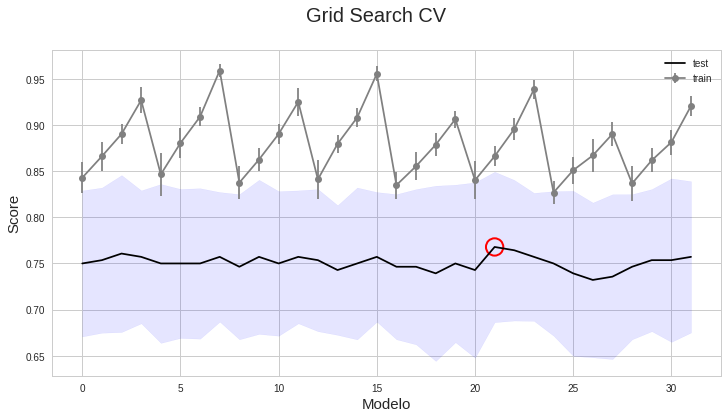
\includegraphics[width=\linewidth]{figure/s_reg_pca.png}\caption{Representación PCA}
\endminipage\hfill
\minipage{0.5\textwidth}
  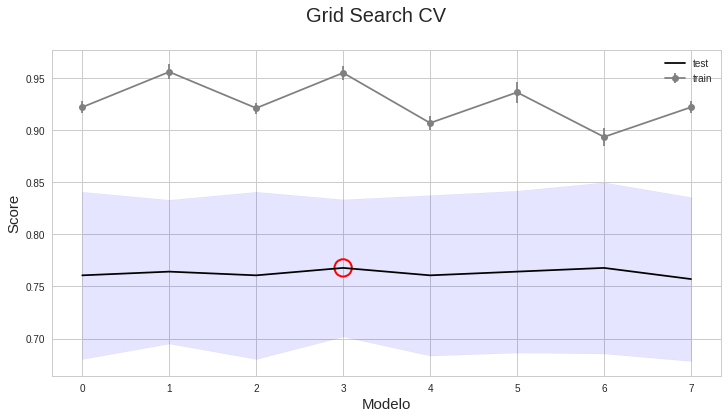
\includegraphics[width=\linewidth]{figure/s_reg.png}
  \caption{Datos reales}
\endminipage
\caption{Score usando K-fold CV y usando un modelo de regresión logística.}\label{s_reg}
\end{figure}

\subsection*{Nuevos modelos de clasificación}
A diferencia del ejercicio anterior, en este ejercicio si se observa una mejoría en el score usando nuevos métodos de clasificación. Por lo cuál, consideramos que es necesario presentar nuevamente todas los efectos en cada uno de los modelos.\\

Los ajustes se hicieron por separado considerando los datos originales o representación PCA, con el objetivo de no saturar la carga computacional. En las representaciones PCA se utilizaron las mismas que en el ejercicio 1.

\subsubsection*{Redes Neuronales}
Consideramos diferentes arquitecturas para las redes neuronales: \textbf{una capa oculta y una neuronal, diez capaz ocultas cada una con una neurona, diez capaz ocultas con diez neuronas y diez capas ocultas con tres neuronas}. También se consideraron diferentes valores para el parámetro de regularización: \textbf{0.1, 0.5 y 0.01}; y también consideramos diferentes funciones de activación: \textbf{relu}. En total se probaron 70 modelos distintos, se probaron primero 35 modelos y posteriormente 70 debido al costo computacional.\\

Los resultados de la validación se pueden observar en las Figuras \ref{s_redes}. La mejor combinación de parametros fue considerando \textbf{diez capas ocultas con diez neuronas cada una usando la función de activación relu con un valor de 0.5 en el parámetro de regularización y utilizando los datos originales, la cual arrojo un score de 0.782.}

\begin{figure}[!htb]
\minipage{0.5\textwidth}
  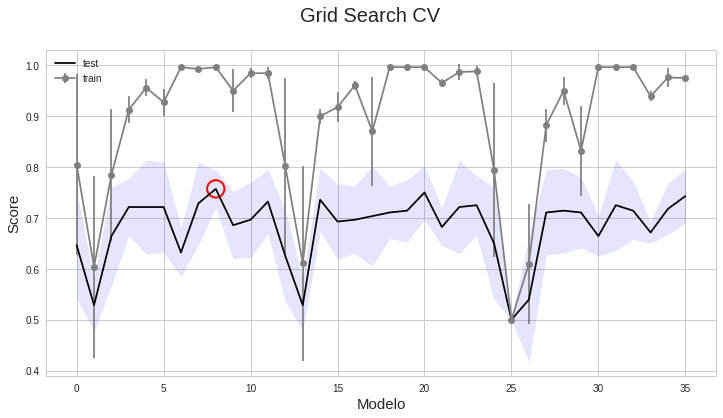
\includegraphics[width=\linewidth]{figure/s_redes_pca.png}
  \caption{Representación PCA.}\label{act}
\endminipage\hfill
\minipage{0.5\textwidth}
  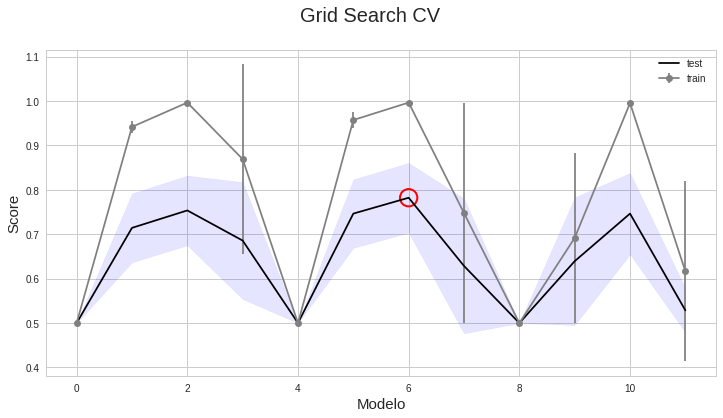
\includegraphics[width=\linewidth]{figure/s_redes.png}\caption{Datos originales.}\label{arqui}
\endminipage
\caption{Score usando K-fold CV y usando redes neuronales.}\label{s_redes}
\end{figure}


\subsubsection*{SVM}
Para este modelo los hyperparametros a controlar fueron el parametro de regularización: \textbf{0.001, 0.01 y 1};   el tipo kernel usando en el algoritmo: \textbf{linear y rbf}; y el coeficiente del kernel (cuando use un kernel rbf): 0.001, 0.01, 0.1, 1, 10 y 100. En total se probaron 83 modelos.\\

Los resultados de la validación cruzada se observa en la Figura \ref{s_smv}. Podemos observar que cuando utilizamos un kernel \textit{rbf} el modelo es malo en comparación con un kernel \textit{linear}. Ahora considerando solo los modelos con un kernel \textit{linear}, podemos observar que entra mayor sea el número de componentes principales a usar el rendimiento es mayor pero es mejor si se consideran todos los datos originales. El efecto del  parámetro de regularización no es tan grande como los otros parámetros considerados. 

\begin{figure}[!htb]
\minipage{0.5\textwidth}
  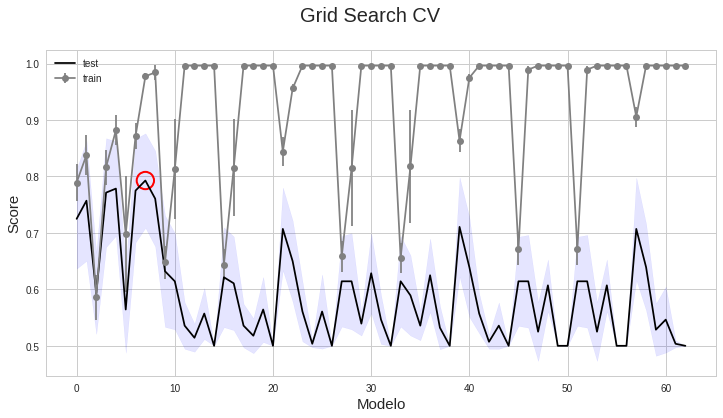
\includegraphics[width=\linewidth]{figure/s_smv_pca.png}
  \caption{Representación PCA.}\label{act}
\endminipage\hfill
\minipage{0.5\textwidth}
  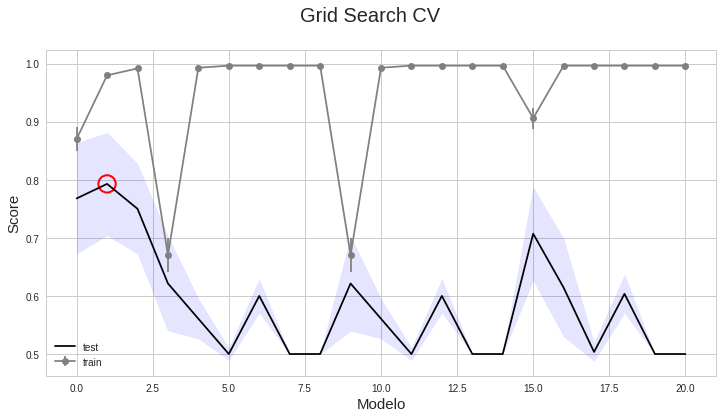
\includegraphics[width=\linewidth]{figure/s_smv.png}\caption{Datos originales.}\label{arqui}
\endminipage
\caption{Score usando K-fold CV y usando SVM.}\label{s_smv}
\end{figure}

\textbf{La mejor combinación de hiperparametros es considerar un kernel linear con un valor de 0.01 en el parametro de regularización y utilizando los datos originales, el cual arroja un score de 0.792.} 


\subsubsection*{Arboles de clasificación}
Para este modelo los hyperparametros a controlar fueron el número de hojas de los arboles: \textbf{2, 3 y 5},  y el número de variables a considerar para realizar la mejor separación: \textbf{auto, sqrt y log2}. En total se probaron 47 modelos.\\

Los resultados de la validación cruzada se observa en la Figura \ref{s_tree}. Para este modelo se observar un efecto muy notorio para los tres parámetros considerados, pero lamentablemente el \textbf{escore máximo de todas las combinaciones posibles es de $0.614$ lo cual es malo en comparación con los resultandos anteriores, el cuál se obtiene utilizando 2 hojas en los arboles y usando el valor log2 en los primeros 80 componentes principales.}

\begin{figure}[!htb]
\minipage{0.5\textwidth}
  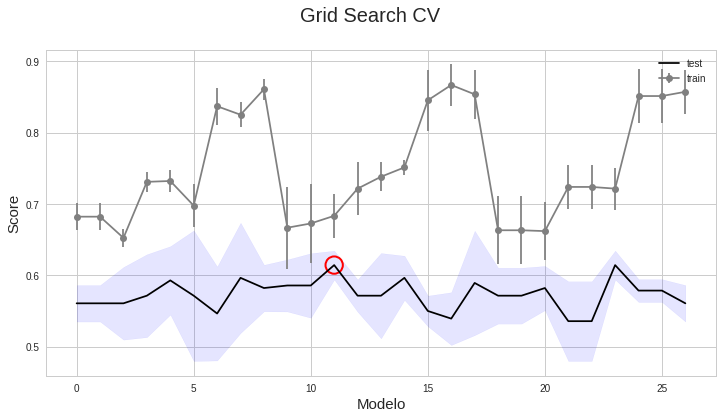
\includegraphics[width=\linewidth]{figure/s_tre_pca.png}
  \caption{Representación PCA.}\label{act}
\endminipage\hfill
\minipage{0.5\textwidth}
  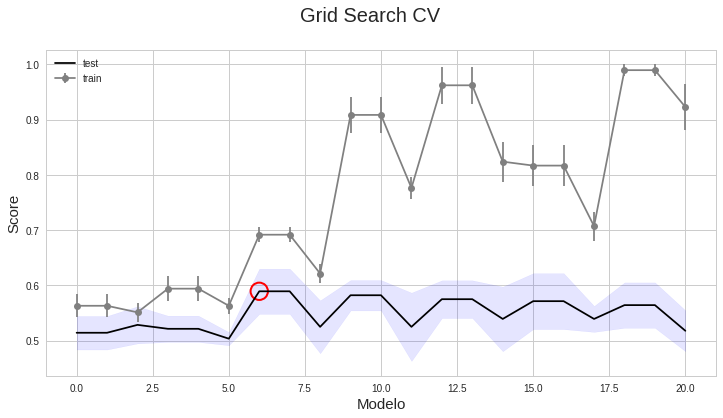
\includegraphics[width=\linewidth]{figure/s_tree.png}\caption{Datos originales.}\label{arqui}
\endminipage
\caption{Score usando K-fold CV y usando Arboles de clasificación.}\label{s_tree}
\end{figure}


\subsubsection*{AdaBoots}
Para este último modelo, los párametros más importantes son el clasificador débil y el número de iteraciones bosting y el algoritmo. Nosotros primero solo controlamos el número de iteraciones: 50, 100 y 200; y el algorimos a usar: SAMME y SAMME.R, estas combinaciones fijamos el clasificador base ocupado un arbol de desición una 1 hoja. Y posteriormente contralamos el clasificador base, el cual consideramos todas las combinaciones del clasificación de los Arboles de clasifiación de la sección anterior.\\

La mejor combinación es considerando\textbf{ 2 hojas en los arboles de desición y considerar un número máximo de variables a considerar log2 considerando el argoritmo SAMME.R y 200 iteraciones, esta combinación nos arrojo un score de 0.6857.}
\begin{figure}[!htb]
\minipage{0.5\textwidth}
 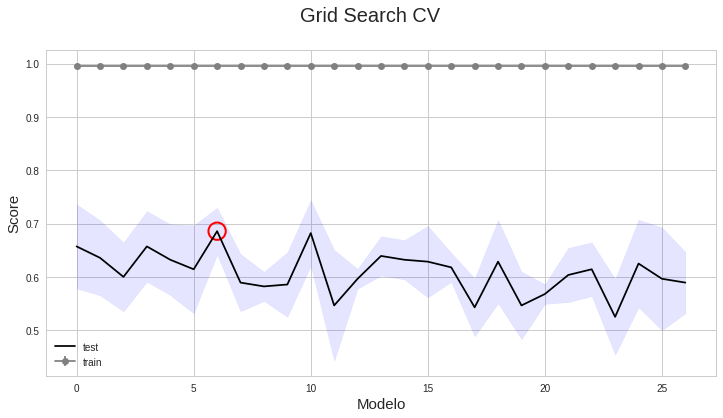
\includegraphics[scale=0.4]{figure/s_ada_pca.png}\caption{Score usando K-fold CV y el modelo AdaBoots.}\label{s_ada_pca}
\endminipage\hfill
\minipage{0.5\textwidth}
  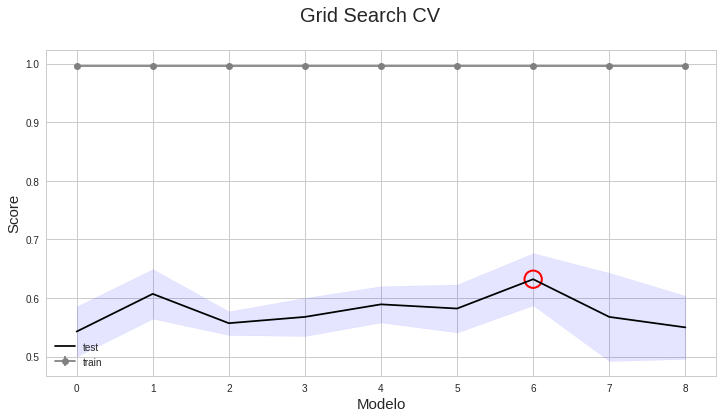
\includegraphics[scale=0.4]{figure/s_ada.png}\caption{Score usando K-fold CV y el modelo AdaBoots.}\label{s_ada}
\endminipage
\caption{Score usando K-fold CV y usando AdaBoots.}\label{s_adas}
\end{figure}


\subsection{Comparación de los mejores modelos}
Si comparamos todos los mejores scores de los diferentes modelos probados anteriormente (ver Cuadro \ref{compa}), podemos observar que los score son muy parecidos pero \textbf{el mejor rendimiento se obtiene usando SVM y en los datos originales.} A diferencia del ejercio anterior, podemos notar que estos modelos si tuvieron mayor rendimieto que los \textit{métodos anteriores}.
\begin{table}[H]
\centering
\begin{tabular}{cccc}
\hline \hline
Model & score &Hiperparámetros &Datos \\
LogReg & 0.7678 &$mutinomial, C=0.0094$& 80 componentes principales\\
Redes neuronales & 0.782 &$[10,10],\ relu,\ C=0.5$&datos originales\\
SVM & 0.792  &$linear, \ C=0.01$ &datos originales\\
Arboles de clasificación & 0.614 & $2\ hojas, log2$& 80 componentes principales\\
ADABoots & 0.6857&$SAMME.R,\ 200,\ 2 \ hojas,\ log2$ &200 componentes principales  \\ \hline \hline 
\end{tabular}
\caption{Comparación de los score usando 5-fold.}\label{compa}
\end{table}
\subsection{Evaluación del mejor modelo en los datos de prueba}
Una vez seleccionado el mejor modelo usando el críterio de validación cruzada, procedemos a calcular las metricas de error para el conjunto de prueba (Ver Cuadro \ref{error_o}). En general podemos notar que las métricas de error están algo bajas, pero considero que son buenas por la complejidad del ejercicio. Es decir, debido a que estamos intentando clasificar apartir de una opinión si es positiva o negativa, es una tarea algo abstracta para un modelo.
\begin{table}[H]
    \centering 
        \begin{tabular}{|c|c|c|c|c}
        \hline
dígito  & precision &  recall & f1$-$score\\
no      &  0.68  &  0.83   & 0.75\\  
yes      &  0.79  &  0.62   & 0.69\\   \hline \hline
accuracy  & & & 0.73\\ \hline \hline
        \end{tabular}
        \caption{Métricas de error para el conjunto de prueba.} \label{error_o}  
\end{table}
Podemos observar que clasificamos más la categoría yes en la mayoría del tiempo, lo que provoca que el error de clasificación en el sentimiento no cresca. Entonces para mejorar el algoritmo, un enfoque sería concentrarnos en clasificar bien las opiniones cuando sean positivas ya que nos cuesta más trabajo identificarlas. (Ver Figura \ref{ocho_o}).
\begin{figure}[H]
\centering
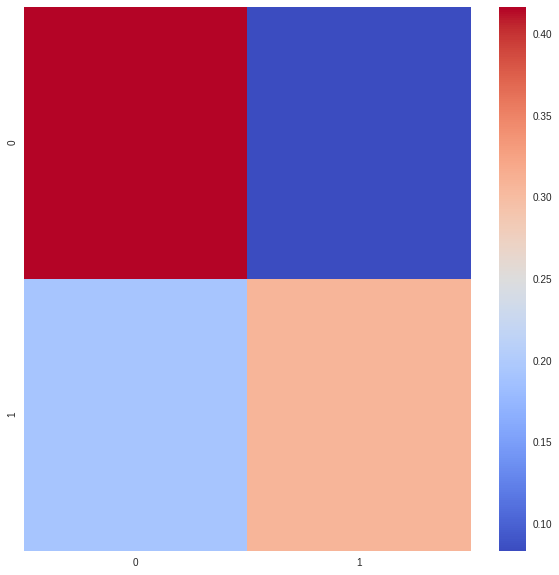
\includegraphics[scale=0.4]{figure/metrica_o.png}
\caption{Matriz de confusión del conjunto de prueba, usando el mejor modelo SVM.}\label{ocho_o}
\end{figure}


\section{Frutas clasificación.}
Para este ejercicios probaremos la eficiencia de los modelos utilizados en el ejercicio 1 para los datos de frutas utilizadas en la tarea 3. \\

Los datos a utilizar es una representación en el espacio HSV con la mediana y los cuartiles centrales, es decir, consideramos 12 variables. Para este ejercicio no utilizamos PCA para reducir la dimensionalidad, debido a que son pocas variables.

\subsection*{Comparación de los modelos}
Consideramos las mismas combinaciones de los ejercicios anteriores, sin considerar el control del número de componentes principales a utilizar. Es decir, para las redes neuronales solo validamos 12 combinaciones (arquitectura de la red y parametro de regularización) de parametros, para SVM (kernel usado, parámetro de regularización y parámetro del kernel en rbf) consideramos 21 combinaciones, para los arboles de decisión consideramos 21 combinaciones (hojas a utilizar y arboles a utilizar) y por último para AdaBoost consideramos 9 combinaciones (clasificador base). Los demás parámetros son los que están por default en las funciones.\\

Los resultados de los 63 modelos se pueden observar en la Figura \ref{futras}. Podemos observar que los mejores clasificadores son considerando los arboles, estos tienen los mejores resultados. Posteriormente el SVM tiene buenos resultados y por último la red neuronal. El mejor clasificador es considerando AdaBoost con 5 hojas en cada arbol y utilizando el número máximo de arboles auto, esta combinación arroja un score de 0.998.

\begin{figure}[H]
\centering
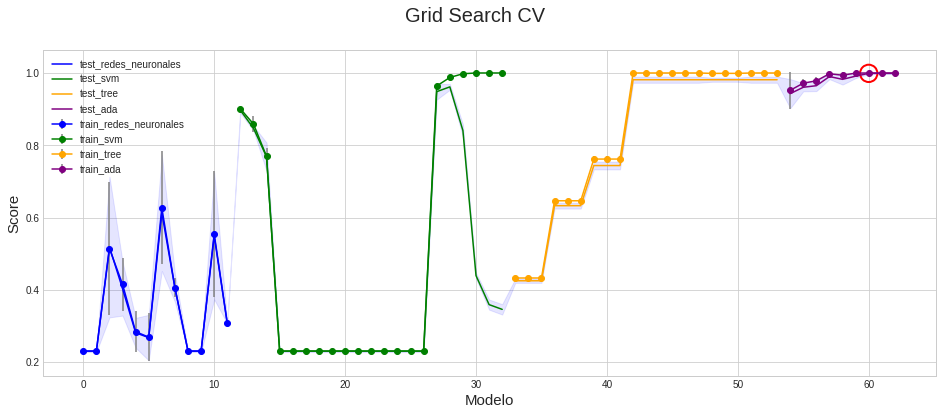
\includegraphics[scale=0.55]{figure/frutas.png}
\caption{Score de los distintos modelos.} \label{futras}
\end{figure}
\subsection{Evaluación del mejor modelo en los datos de prueba}
Una vez seleccionado el mejor modelo usando el críterio de validación cruzada, procedemos a calcular las metricas de error para el conjunto de prueba (Ver Cuadro \ref{error_o}). Podemos observar que la clasificación para el conjunto de prueba es perfecto, el clasificador no se equivoco en ninguna frtua. 
\begin{table}[H]
    \centering 
        \begin{tabular}{|c|c|c|c|c}
        \hline
fruta      & precision &  recall & f1$-$score\\
Apricot     &  1.00  &  1.00   & 1.00\\  
Avocado     &  1.00  &  1.00   & 1.00\\  
Carambula   &  1.00  &  1.00   & 1.00\\  
Cherry      &  1.00  &  1.00   & 1.00\\  
Huckleberry &  1.00  &  1.00   & 1.00\\  
Kiwi        &  1.00  &  1.00   & 1.00\\  
Orange      &  1.00  &  1.00   & 1.00\\  
Peach       &  1.00  &  1.00   & 1.00\\  
Pineapple   &  1.00  &  1.00   & 1.00\\  
Strawberry  &  1.00  &  1.00   & 1.00\\  
Apple  		&  1.00  &  1.00   & 1.00\\  \hline \hline
accuracy  & & & 1.00\\ \hline \hline
        \end{tabular}
        \caption{Métricas de error para el conjunto de prueba.} \label{error_o}  
\end{table}
Por lo que podemos concluir que nuestro clasificador es muy bueno.
\subsection{Conclusión}
En conclusión (no solo de este ejercicio, sino de toda la tarea), podemos observar que los diferentes métodos de clasificación son buenos para distintos problemas. \textbf{Claramente observamos en los ejercicios 1 y 2 que los arboles de clasificación y AdaBoost eran muy malos. En cambio en este último ejercicio fueron los modelos que tuvieron mejores resultados.}\\

Además, este ejercicio nos enseño a poder utilizar validación cruzada de forma correcta para no cometer algún sesgo con el conjunto de datos de entrenamiento lo cual es de suma importancia.

\section{Anexos}
Todos los códigos utilizados para estos resultados se pueden encontrar en mi página personal de Gitgub: Enriquesec. En el repositorio Ciencia de Datos/Tareas/Tareas$_$6/. El notebooks solutions.ipynb contiene las soluciones del ejercicio 1 y 3, y el notebooks solutions2.ipynb contiene las soluciones del ejercicio 2.

\printbibliography


\end{document}
